\section{Illustrative substitution configurations}
\label{app:trajectory}

This appendix shows what the labor account returns for chosen substitution fractions. It is an
arithmetic illustration of Section~\ref{sec:workforce}, not an estimated trajectory or a forecast
calendar. Take the 140 people of Table~\ref{tab:populations} with $K=120$ hours per month and full
allocation across the three routes. Table~\ref{tab:allocation} gives an assumed split of each
population's baseline FTE between W1, W2, and W3. The modeled pool is the buying and integrating
enterprise's governance workforce; supplier-side production in Buy requires a separately measured
supplier account.

\begin{table}[!htb]
\centering\small
\caption{Synthetic populations shared across the three workflows. The route columns are allocated
baseline FTE, not additional employees.}
\label{tab:allocation}
\begin{tabular}{@{}l l r r r r@{}}
\toprule
Pool & Population & Baseline & W1 & W2 & W3\\
\midrule
\rowsinput{generated/table_allocation_rows}
\bottomrule
\end{tabular}
\end{table}

Let $a_w$ be the fraction of baseline case-processing labor displaced on route $w$, after counting
remaining case review and rework, and $F$ additional shared human support in FTE. Then
\begin{equation}
N_A = 51.25(1-a_1)+36(1-a_2)+52.75(1-a_3)+F. \label{eq:trajectory}
\end{equation}
The uneven-substitution row of Table~\ref{tab:trajectory} leaves 30\%, 75\%, and 25\% of baseline route
labor, reflecting the route order proposed in Section~\ref{sec:milestones}; the advanced row leaves
5\%, 20\%, and 3\%. Each uses five shared support FTE. The final rows distinguish completion of direct
gate execution from closure of its remaining support work. Totals use unrounded values and are
displayed rounded half up.

\begin{table}[!htb]
\centering\small
\caption{Required human workload (FTE-equivalent) in illustrative substitution configurations. All
three workflows remain in the process.}
\label{tab:trajectory}
\begin{tabular}{@{}l r r r r r@{}}
\toprule
Operating configuration & W1 & W2 & W3 & Support & Total\\
\midrule
\rowsinput{generated/table_trajectory_rows}
\bottomrule
\end{tabular}
\end{table}

\begin{figure}[!htb]
\centering
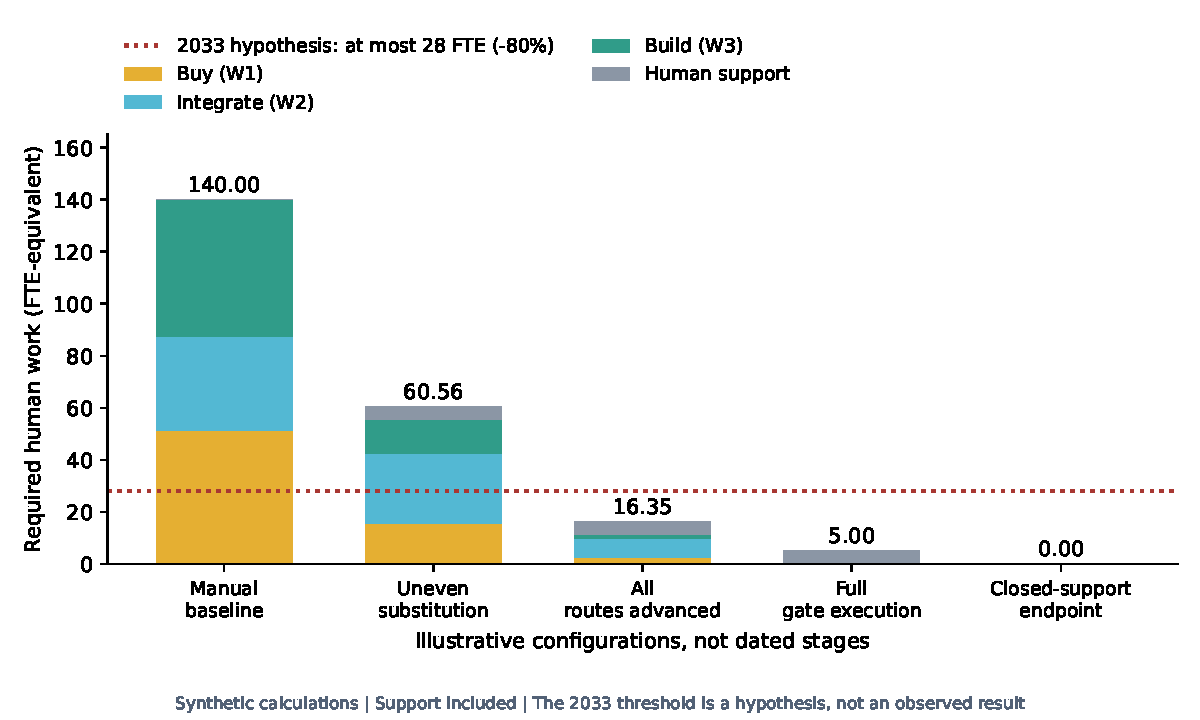
\includegraphics[width=0.84\linewidth]{figures/fig_trajectory.pdf}
\caption{\textbf{The workflows remain; their execution workforce contracts.} Route contributions are
shown separately and the shared human-support term is counted once. The final zero is the consequence
of complete closure assumed in that configuration, not a measured capability or a predicted date.
The dotted 28-FTE line marks the separate 2033 hypothesis: 80\% below the illustrative 140-FTE
baseline, support included. The bars are configurations, not a calendar trajectory.}
\label{fig:trajectory}
\end{figure}

With common labor displacement $a$ across routes, Equation~\eqref{eq:trajectory} becomes
$N_A=140(1-a)+F$. Table~\ref{tab:floor} shows how a support floor determines the endpoint.

\begin{table}[!htb]
\centering\small
\caption{Residual required FTE under common labor displacement and alternative human-support floors.
These are conditional arithmetic values.}
\label{tab:floor}
\begin{tabular}{@{}r r r r@{}}
\toprule
Labor displaced & No support floor & 5 FTE floor & 15 FTE floor\\
\midrule
\rowsinput{generated/table_floor_rows}
\bottomrule
\end{tabular}
\end{table}
